\chapter{Robótica de enxame}
\label{swarm}

\section{Introdução}

Observando os seres vivos presentes na natureza, podemos facilmente extrair algumas qualidades que estes apresentam: flexibilidade, robustez, descentralização, auto-organização. Em grande parte, o motivo por trás dessas qualidades é a coletividade. Por exemplo, em colônias de insetos sociais, diversos indivíduos se auto-organizam para realizar tarefas cuja  escala e complexidade superam, e muito, os limites físicos e cognitivos de cada indivíduo \cite{navarro2012introduction}. Podemos visualizar uma colônia como um único super-organismo \cite{trianni2011swarm} e podemos interpretar inteligência como uma característica que emerge das interações entre componentes simples e interdependentes de um sistema.

Sob esse ponto de vista, uma série de algoritmos computacionais têm sido propostos em uma área de pesquisa denominada inteligência coletiva (\textit{swarm intelligence}) \cite{bonabeau1999swarm} \cite{kennedy2001swarm}. Da mesma forma, a área denominada robótica de enxame (\textit{swarm robotics}) estuda como grupos de agentes relativamente simples podem ser projetados a fim de resultar em um determinado comportamento coletivo a partir de interações entre os próprios agentes e os agentes e o ambiente \cite{sahin2005swarm}.

\section{Comportamentos coletivos}

Na literatura da área encontram-se diversos comportamentos coletivos a serem reproduzidos no contexto da robótica. Alguns relativamente simples e outros bastante mais complexos, que em geral dependem da execução coordenada de alguns dos comportamentos coletivos simples.

O comportamento de \textbf{agregação}, por exemplo, consiste simplesmente na reunião dos robôs do enxame e é utilizado por outros comportamentos complexos, como o movimento coletivo, a auto-montagem e a formação de padrões, nos quais em determinados momentos o enxame se reúne.

No comportamento de \textbf{dispersão}, o enxame se distribui de modo a ocupar a maior área possível do espaço sem perder comunicação. É útil em tarefas que envolvam a exploração coletiva de um território desconhecido.

A \textbf{formação de padrões} é um comportamento em que os robôs devem movimentar-se de maneira coordenada para distribuírem-se no espaço segundo um determinado modelo de posicionamento.

Já no comportamento de \textbf{movimento coletivo} o enxame deve mover-se em conjunto e de maneira coesa \cite{sperati2008evolving}. Há, nesse caso, uma clara inspiração na natureza, por exemplo na maneira como se movimentam pássaros em um bando ou peixes em um cardume. Pelo menos dois tipos de movimento coletivo podem ser identificados: \textbf{formation}, em que o posicionamento e a orientação dos robôs mantêm-se fixa, e \textbf{flocking}, em que isso não acontece.

O comportamento de busca por alimento (\textbf{foraging}) observado na natureza pode inspirar uma gama mais ampla de problemas em que os robôs devem encontrar as coordenadas de um ponto do ambiente com características definidas.

A \textbf{formação de caminho} é uma variação de movimento coletivo que também se enquadra em busca por alimento. Visa o trajeto do enxame pelo menor caminho entre dois pontos, assim como, na natureza, as formigas utlizam de feromônios para encontrar e navegar pelo menor caminho entre o formigueiro e alguma fonte de alimento.

\textbf{Alocação de tarefas} é um comportamento genérico que se aplica a diversos problemas em que o enxame precisa, de maneira coletiva e descentralizada, definir a tarefa que cabe a cada robô. Trata-se de um problema relativamente complexo em que diversos estudos vêm sendo realizados.

O \textbf{transporte coletivo} de objetos é outro comportamento facilmente observável na natureza também em colônias de formigas. Envolve alto grau de coordenação e depende de vários dos comportamentos básicos mais simples \cite{gross2006autonomous}.

Um comportamento com importante aplicação na exploração de ambientes desconhecidos é o do \textbf{mapeamento coletivo}, em que o comportamento de dispersão é associado à troca de informações entre robôs com o objetivo de produzir uma representação mais ampla do ambiente.

Outro comportamento relativamente complexo é a \textbf{auto-montagem} \cite{christensen2007mechanism}, que consiste na agregação e interconexão de robôs formando padrões que podem ser posteriormente utilizados para a solução coletiva de problemas.

\section{Formação de caminho}

Da observação do comportamento de diversas espécies de formigas, nota-se o uso de químicos (feromônios) para estabelecer uma forma de comunicação que permite: o recrutamento em massa de indivíduos e a formação dinâmica de um caminho para transporte do alimento para dentro da colônia.

No contexto de robótica de enxame, Fujisawa et al. \cite{fujisawa2008pheromone} recria com sucesso esse comportamento em um grupo de robôs. No entanto, a síntese, armazenamento, fator de evaporação e detecção confiável dos quimícos não é nada simples e dificulta o uso prático de tal método.
Por outro lado, diversas abordagens ao problema procuram alternativas aos feromônios, por exemplo: projeção luminosa \cite{garnier2007alice}, \textit{RFID}\footnote{\textit{Radio-frequency identification -- Identificação por radiofrequência.}} \cite{mamei2007rfid}, trilhas virtuais \cite{payton2001pheromone} etc.

Neste trabalho focaremos no seguinte problema: recriar o comportamento de formação de caminho de forma eficiente -- entende-se menor caminho -- entre duas áreas alvo por um enxame de robôs. A posição de cada área alvo é aleatória e desconhecida pelos robôs. A Figura \ref{fig:path-formation} apresenta um exemplo de instância do problema.

\begin{figure}[H]
    \centering
    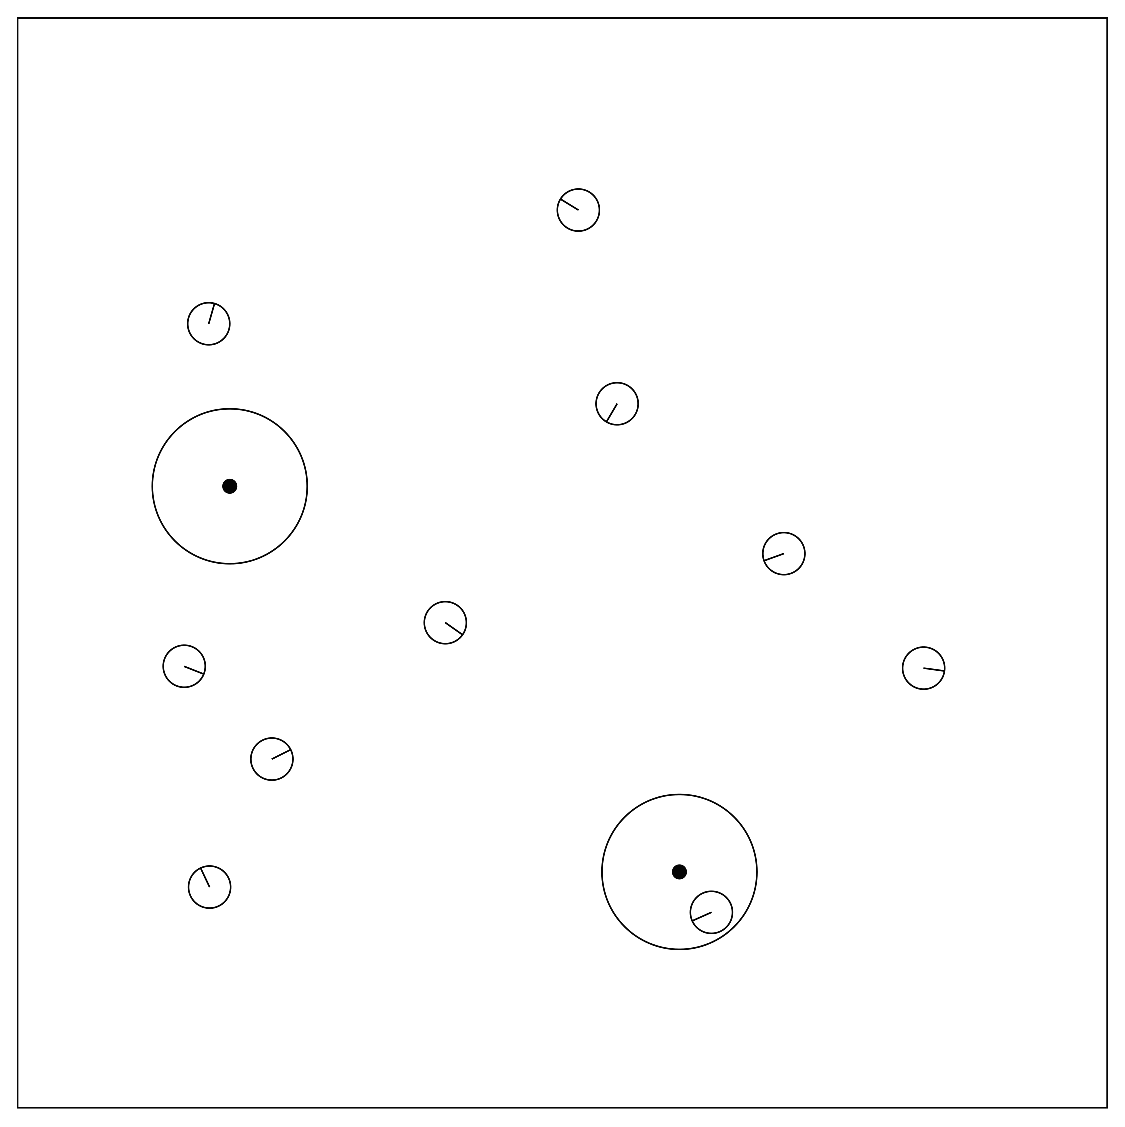
\includegraphics[width=0.5\textwidth]{figures/path-formation}

    \caption{Exemplo de instância do problema de formação de caminho com 10 robôs. As duas circunferências maiores representam as áreas alvo e as menores representam os robôs.}
    \label{fig:path-formation}
\end{figure}